\documentclass[12pt,french]{report}

% This is the main framework I use for my LateX documents.
% main.tex by Alexis GRACIAS, last modification 21 November, 2024

%%%%%%%%%%%%
% PACKAGES %
%%%%%%%%%%%%

% GEOMETRY

\usepackage[left=2cm,right=2cm,top=2cm,bottom=2cm]{geometry}

% LANGUAGE

\usepackage{babel}

% REFERENCES

\usepackage{hyperref} % Add links to the table of content, files and website

% GRAPHS

\usepackage{tikz} % Graph package

% IMAGES

\usepackage{graphicx} % Required for inserting images
\usepackage{tabto}

% COLOR

\usepackage[skins,theorems]{tcolorbox} % Frame color package
\usepackage{amssymb}
\usepackage[dvipsnames]{xcolor} % Text color package and more colors

% Custom colors
\definecolor{ao}{rgb}{0.0, 0.0, 1.0}
\definecolor{coolblack}{rgb}{0.0, 0.18, 0.39}
\definecolor{cyan}{rgb}{0.0, 1.0, 1.0}
\definecolor{glaucous}{rgb}{0.38, 0.51, 0.71}
\definecolor{electricultramarine}{rgb}{0.25, 0.0, 1.0}


% CAPTIONS

\usepackage{caption}
\usepackage{subcaption}
\usepackage[utf8]{inputenc}

% OTHER

\usepackage{pdfpages}

% MATH

\usepackage{amsmath,amsfonts,mathtools,stmaryrd} % Math libraries

\usepackage{listings} % required for specific languages
\lstset{ % Set listing package options
    language=bash, % choose the language of the code
    basicstyle=\fontfamily{pcr}\selectfont\footnotesize\color{red},
    keywordstyle=\color{black}\bfseries, % style for keywords
    numbers=none, % where to put the line-numbers
    numberstyle=\tiny, % the size of the fonts that are used for the line-numbers     
    backgroundcolor=\color{white},
    showspaces=false, % show spaces adding particular underscores
    showstringspaces=false, % underline spaces within strings
    showtabs=false, % show tabs within strings adding particular underscores
    frame=single, % adds a frame around the code
    tabsize=2, % sets default tabsize to 2 spaces
    rulesepcolor=\color{gray},
    rulecolor=\color{black},
    captionpos=b, % sets the caption-position to bottom
    breaklines=true, % sets automatic line breaking
    breakatwhitespace=false, 
}

%\usepackage{eso-pic,lipsum}
%\AddToShipoutPicture{%
%	\AtTextCenter{%
%		\fboxsep5mm \fboxrule=0.8pt
%		\makebox(0,0)[c]{\fbox{\rule{0pt}\textheight\rule\textwidth{0pt}}}%
%	}%
%}

%%%%%%%%%%%%
% COMMANDS %
%%%%%%%%%%%%

\lstset{aboveskip=\baselineskip,belowskip=\baselineskip,basicstyle=\ttfamily} % Formating line break after bash commands

% Get rid of 0. chapter's number
\makeatletter 
\renewcommand{\thesection}{%
  \ifnum\c@chapter<1 \@arabic\c@section
  \else \thechapter.\@arabic\c@section
  \fi
}
\makeatother

% Rules for \bar{x} and \overline{x} commands
\makeatletter
\newcommand*{\Xbar}{}%
\DeclareRobustCommand*{\Xbar}{%
  \mathpalette\@Xbar{}%
}

% THEOREMS

\tcbuselibrary{theorems} 
\newtcbtheorem
  []% init options
  {definition}% name
  {Definition}% title
  {%
    colback=electricultramarine!5,
    colframe=electricultramarine!35!black,
    fonttitle=\bfseries,
  }% options
  {def}% prefix

% FORMULAS

\tcbset{highlight math style={enhanced,
  colframe=red,colback=white,arc=0pt,boxrule=1pt}}

% CUSTOM COMMANDS

\newcommand*{\@Xbar}[2]{%
  % #1: math style
  % #2: unused (empty)
  \sbox0{$#1\mathrm{X}\m@th$}%
  \sbox2{$#1X\m@th$}%
  \rlap{%
    \hbox to\wd2{%
      \hfill
      $\overline{%
        \vrule width 0pt height\ht0 %
        \kern\wd0 %
      }$%
    }%
  }%
  \copy2 %
}
\makeatother

%%%%%%%%%%%%%%%%%%%%%%
% DOCUMENTS SETTINGS %
%%%%%%%%%%%%%%%%%%%%%%
% Fist page
\title{\Huge Fiche de révision Traitement Audio}
\author{\LARGE Alexis GRACIAS}
\date{\Large \today}

% Document
\begin{document}
\maketitle
\large \tableofcontents

\normalsize

%%%%%%%%%%%
% INCLUDE %
%%%%%%%%%%%
\chapter*{Introduction}


\chapter{Les sons - Modèle de perception}
\section{Introduction}
\subsection{Définitions}
\begin{itemize}
    \item \textbf{Psychophysique} : relation entre le \textit{stimulus}\footnote{Phénomène physique} et la \textit{sensasion} ressentie du stimulus. \newline
    \item \textbf{Psychoacoustique} \footnote{Remarque : on peut tromper l'ouie comme la vue, avec des sons appelés \textbf{sons de Risset}} : étude de la relation entre les vibrations des ondes sonores et sa perception.\newline
    \item \textbf{Les modèles de production} permettent de caractériser les osurces dans la nature.
\end{itemize}
\subsection{Histoire des sens} \footnote{D'après Ch. Sherrington (1857-1952)}
\begin{itemize}
    \item Les sens \textit{introseptifs} : sensations qui vienne des entrailles du corps (estomac, coeur, malaise, aise...)
    \item Les sens \textit{Proprioceptifs} : 
        \begin{itemize}
            \item Sens \textit{statique} ou \textit{labyrinthique}\footnote{Provient du "capteur" situé dans l'oreille interne} : mouvements de rotation et de translation
            \item Sens \textit{kinésique} ou \textit{kinestésique} : permet la perception des objets dans l'espace, par exemple le toucher
        \end{itemize}
    \item Les sens \textit{extéroceptifs}
        \begin{itemize}
            \item Sens par contact direct
                \begin{itemize}
                    \item Le \textit{toucher}
                    \item Les sens \textit{chimique} : goût, odorat
                \end{itemize}
            \item Sens par contact indirect
                \begin{itemize}
                    \item \textit{Vue}
                    \item \textit{Ouie}
                \end{itemize}
        \end{itemize}
\end{itemize}
\newpage
\subsection{Lois des sens (18ème - 19ème)}
\begin{itemize}
    \item \textbf{Loi du sens} : il existe pour chaque sens une intensité minima du stimulus, appelée intensité liminaire, au-dessous de laquelle il n'y a pas de sensation
    \item \textbf{Loi du seuil différentiel} : 
        \begin{itemize}
            \item Forme a. \newline
            Il existe un rapport constant entre l'intensité du stimulus initial et la variation minima qu'il faut lui faire subir pour que la différence soit sentie
            \item Forme b. \newline
            Pour que la sensation subisse des accroissements en progression arithmétique (0, 1, 2...), il faut faire varier le stimulus en progression géométrique (a, a2, a3...) ; le rapport constant est le seuil liminaire. C'est encore la loi logarithmique, ou loi de Fechner
        \end{itemize}
\end{itemize}
\newpage
\section{Stimulus auditif : le son}
\subsection{Qu'est-ce que le son ?}
C'est la sensation perçue par l'oreille. Variation périodique de la pression d'un milieu.
\subsection{Hypothèses du cours}
\begin{itemize}
    \item Millieux de propagation \footnote{(gazs, liquides, solides)} supposés parfaits, sans viscosité et au repos \footnote{En réalite, pour les fluides visqueux, on doit résoudre l'équation de Navier-Stokes par la méthode des éléments finis}
    \item Vibrations de faible amplitude
    \item Transformations des fluides supposés adiabatiques réversibles
\end{itemize}
\subsection{Equation d'ondes unidimensionnelle}
Equation de propagation des ondes électro-magnétiques :
\begin{equation}
    \large
    \tcbhighmath[fuzzy halo=0.5mm with electricultramarine!35!electricultramarine,arc=2pt,
    boxrule=0pt,frame hidden]{ 
        \frac{\partial^{2} \psi}{\partial t^{2}} = c_{s}^{2}\frac{\partial^{2} \psi}{\partial x^{2}}
     } \nonumber
    \normalsize
\end{equation}
et : 
\begin{equation}
    \label{eq 1}
    \rho_{e} = -\rho_{0}\frac{\partial \psi }{\partial x}  
\end{equation}
\begin{equation}
    \label{eq 2}
    P_{e} = c_{s}^{2}\rho_{e}
\end{equation}
\begin{equation}
    \label{eq 3}
    \rho_{0} \frac{\partial^{2} \psi}{\partial t^{2}} = -\frac{\partial P_{e}}{\partial x}
\end{equation}
Ce qui devient pour l'équation d'ondes sonores :
\begin{equation}
    \Large
    \tcbhighmath[fuzzy halo=0.5mm with electricultramarine!35!electricultramarine,arc=2pt,
    boxrule=0pt,frame hidden]{ 
        \frac{\partial^{2} P_{e}}{\partial t^{2}} = \frac{1}{c_{s}^{2}}\frac{\partial^{2} P_{e}}{\partial x^{2}}
     } \nonumber
    \normalsize
\end{equation}
\vfil
\begin{equation}
    \large
    \tcbhighmath[fuzzy halo=0.5mm with electricultramarine!35!electricultramarine,arc=2pt,
    boxrule=0pt,frame hidden]{ 
        c_{s} = 331,4\sqrt{1+\frac{T}{T_{0}}}
     } \nonumber
    \normalsize
\end{equation}
\vfill
\begin{center}
    \small{Pour démonstration voir annexe \ref{Annexe 1}}
\end{center}
\newpage
\subsection{Equation d'ondes en tridimensionnel}
L'équation d'ondes s'écrit à l'aide du d'Alembertien : 
\begin{definition}{D'Alembertien}{d'Alembertien}
    \[ \Xi = \nabla^{2} - \frac{1}{c_{2}^{2}}\frac{\partial^{2}}{\partial t^{2}} \] Avec  : \[ \Xi P_{e} = 0 \]
\end{definition}
Soit :
\begin{equation}
    \large
    \tcbhighmath[fuzzy halo=0.5mm with electricultramarine!35!electricultramarine,arc=2pt,
    boxrule=0pt,frame hidden]{ 
        \nabla^{2}P_{e} - \frac{1}{c_{2}^{2}}\frac{\partial^{2} P_{e}}{\partial t^{2}} = 0 \nonumber
     } \nonumber
    \normalsize
\end{equation}
Avec : \newline
\large
\begin{itemize}
    \item $\nabla^{2}\psi = \Delta \psi = \frac{\partial^{2} \psi}{\partial x^{2}} + \frac{\partial^{2} \psi}{\partial y^{2}} + \frac{\partial^{2} \psi}{\partial z^{2}} + \frac{\partial^{2} \psi}{\partial t^{2}}$ \newline
    \item $\psi$ : fonction d'onde (électromagnétique) \newline
    \item $c_{s}$ : célérité du son dans l'air en $m.s^{-1}$ ($c_{s} \approx 340 m.s^{-1}$) \newline
    \item $P_{e}$ : pression acoustique en $Pa$ \newline
    \item $T$ : température en $C$ \newline
    \item $T_{0} = 273 C$
\end{itemize}
\normalsize
\vfil
Quelques rappels : 

\begin{equation}
    \normalsize
    \tcbhighmath[fuzzy halo=0.5mm with electricultramarine!35!electricultramarine,arc=2pt,
    boxrule=0pt,frame hidden]{ 
        \lambda = cT = \frac{c}{f}
     } \nonumber
    \normalsize
\end{equation}
\begin{itemize}
    \item $c$ : célérité de la lumière ($c = 3.10^{8} m.s^{-1}$)
    \item $T$ : période en $s$
    \item $f$ : fréquence en $Hz$
\end{itemize}
\newpage

\chapter{Marchés et régulations}
\section{La concurrence en Europe}
La politque globale de l'Europe est de mettre en place la concurrence partout ou cela est possible. En effet, la mise en concurrence des entreprises permet de faire baisser les prix pour les consommateurs et donc de réduire l'inflation. Cependant, la concurrence parfaite n'existe pas. Il faut donc que l'Europe puisse appliquer plusieurs politiques pour \textbf{réguler} ces phénomènes. Il y a une surveillance des insitutions visant à réduire les "monopoles naturels", à instaurer des politiques environnementales... \newpage

\subsection{Loi de l'offre et la demande}
\begin{center}
    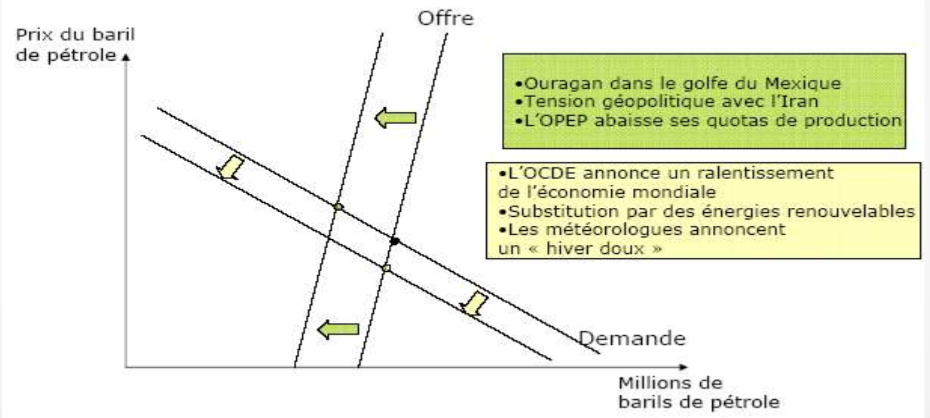
\includegraphics[scale=0.7]{Pics/Offre_et_demande.png}    
\end{center}
$(Offre \searrow + demande = cste) \implies Prix \nearrow$ \newline
$(Offre \nearrow + demande = cste) \implies Prix \searrow$ \newline
$(Demande \searrow + offre = cste) \implies Prix \searrow$ \newline
$(Demande \nearrow + offre = cste) \implies Prix \nearrow$
\subsection{Courbe de l'offre en situation de concurrence}
\begin{center}
    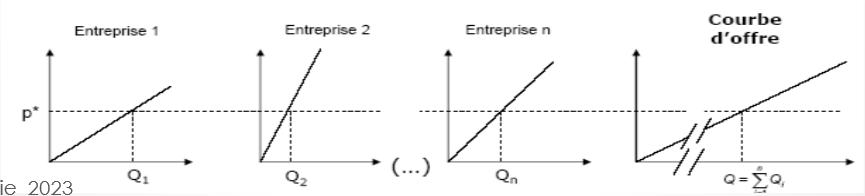
\includegraphics[scale=0.8]{Pics/Courbe_de_l_offre.png}
\end{center}
\newpage
\subsection{Elasticité-prix $\epsilon$ de la demande}
\begin{center}
    \fbox{\huge{$\epsilon = \frac{\frac{dQ}{Q}}{\frac{dp}{p}} = \frac{dQ}{dp}\frac{p}{Q}$}}   
\end{center}
Mesure de la variation de la quantité d'un produit par rapport à la variation de son prix
p : prix du produit \newline
q : quantité du produit
\begin{itemize}
    \item $\epsilon = 0 $ : inélasticité
    \item $\epsilon \in [-1;0[$ : faiblement élastique
    \item $\epsilon \in ]-\infty;-1]$ : élastique
\end{itemize}
\subsection{Elasticité à court et à long terme}
Il faut un certain  temps avant que la quantité d'un produit se stabilise face à une variation de prix
\begin{center}
    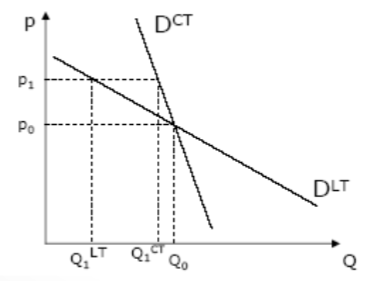
\includegraphics[scale = 1]{Pics/elasticite_court_et_long_terme.png}
\end{center}
\newpage
\subsection{Elasticité des prix croisés de la demande}
C'est la mesure de la déportation d'un produit A vers un produit B lorsque le prix de A augmente.
\begin{center}
    \huge{\fbox{$\epsilon_{i,j} = \frac{\frac{\partial Q_{i}}{Q_{i}}}{\frac{\partial p_{j}}{p_{j}}}=\frac{\partial Q_{i}}{\partial p_{j}}\frac{p_{j}}{Q_{j}}$}}
\end{center}
\begin{itemize}
    \item Si $\epsilon_{i,j} > 0 $: les biens sont substituables
    \item si $\epsilon_{i,j} < 0 $: les biens sont complémentaires
\end{itemize}
\begin{center}
    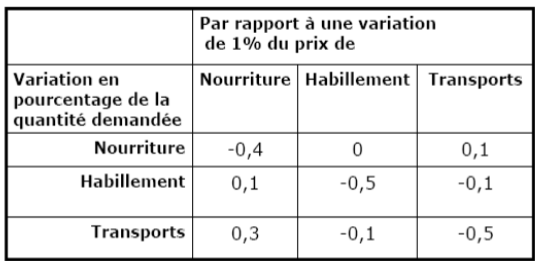
\includegraphics[scale=0.8]{Pics/elasticite_prix_croises.png}
\end{center}
\subsection{Elasticité revenu de la demande}
C'est la mesure de l'évolution du revenu réel du consommateur et de l'évolution de la quantité de produit.
\begin{center}
    \huge{\fbox{$\epsilon_{R} = \frac{\frac{dQ}{Q}}{\frac{dp}{p}}=\frac{dQ}{dp}\frac{p}{Q}$}}
\end{center}
\begin{itemize}
    \item Si $\epsilon_{R} > 1 $: le bien est dit \textbf{de luxe}
    \item si $\epsilon_{R} < 0 $: les biens est dit \textbf{inférieur}
\end{itemize}
\newpage
\section{La technologie de l'entreprise}
Conditions de production de l'entreprise :
\begin{itemize}
\item facteurs de production : 
    \begin{itemize}
        \item $K$ : capital\footnote{Ex : nombre d'heures de fonctionnenment des machines}
        \item $L$ : travail \footnote{Ex : nombre d'heures de travail}
        \item w : taux de salaire horraire
        \item r : coût horraire du capital
    \end{itemize}
\item Fonction de production
    \begin{itemize}
        \item $Q = f(K,L)$
    \end{itemize}
\item Fonction coût de l'entreprise
    \begin{itemize}
        \item $CF$ : coût fixe
        \item $CV(Q)$ : coût variable
    \end{itemize}
\end{itemize}
Fonction de coût total :
\begin{center}
    \Large{\fbox{$CT(Q) = CF + CV(Q)$}}
\end{center}
Fonction de coût moyen :
\begin{center}
    \Large{\fbox{$CM(Q) = \frac{CT(Q)}{Q} = \frac{CF}{Q} + \frac{CV(Q)}{Q}$}}
\end{center}
Fonction de coût marginal :
\begin{center}
    \Large{\fbox{$Cm(Q) = \frac{dCT(Q)}{dQ} = \frac{dCV(Q)}{dQ}$}}
\end{center}
\newpage
\section{Concurrence parfaite}
Comportement de la firme en situation de concurrence :
\begin{itemize}
    \item $\pi$ : profit de l'entreprise
\end{itemize}
Maximisation du profit de l'entreprise, en situation de \textbf{price taker}\footnote{L'entreprise est "preneuse de prix" : elle n'a pas le pouvoir d'influencer les prix sur le marché} : 
\begin{center}
    \Large{\fbox{$\max \pi (Q) = pQ - CT(Q)$}}
\end{center}
Condition de premier ordre :
\begin{center}
    \Large{\fbox{$\frac{d\pi(Q)}{dQ} = 0$}}
\end{center}
\begin{center}
    \Large{$\frac{d\pi(Q)}{dQ} = p - \frac{dCT(Q)}{dQ} = 0 \Longleftrightarrow p - C_{m}(Q) = 0$}
\end{center}
L'entreprise produit une quantité \textbf{à l'équilibre en situation de concurrence parfaite} $Q$ tq :
\begin{center}
    \Large{\fbox{$p=C_{m}(Q)$}}    
\end{center}


Comportement des entreprises sur un marché : plus il y a des opportunités dans un secteurs, plus les entreprises vont vouloir entrer dans ce secteur, ce qui a pour conséquences d'augmenter l'offre et donc de faire baisser les prix. \newline
Conditions de la concurrence parfaite:
\begin{center}
    \begin{itemize}
    \item Atomicité
    \item Biens homogènes
    \item libre entrée
    \item information parfaite
    \item Biens exclusifs
\end{itemize}
\end{center}
\newpage
\subsection{Dynamique de la concurrence parfaite}
Au bout d'un temps suffisament long, les profits $\pi$ des entreprises sont nuls et $p=CM=C_{m}$
\begin{center}
    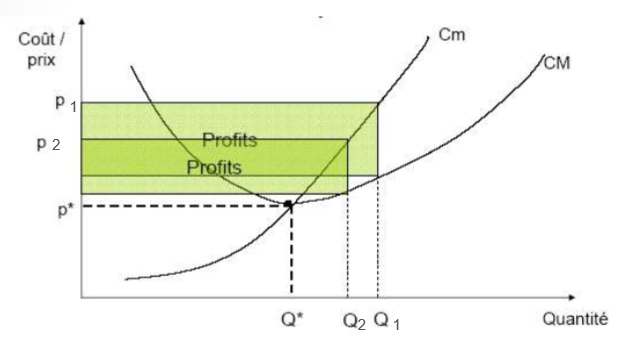
\includegraphics[scale=0.8]{Pics/dyn_concu_parfaite.png}
\end{center}
Rendements de la fonction de production : \newline
La fonction de production a 
\begin{itemize}
    \item Un rendement constant si :
    \begin{center}
        \Large{\fbox{$\lambda Q = f(\lambda K, \lambda L)$ avec $\lambda>1$}}
    \end{center}
    \item Un rendement décroissant si :
    \begin{center}
        \Large{\fbox{$\lambda Q < f(\lambda K, \lambda L)$}}
    \end{center}
        \item Un rendement croissant si :
    \begin{center}
        \Large{\fbox{$\lambda Q > f(\lambda K, \lambda L)$}}
    \end{center}
\end{itemize}
Fonction à rendement constant (fonction de Cobb-Douglas)
\begin{center}
    \Large{$Q = K^{\alpha}L^{\alpha}$}
\end{center}
\newpage
\subsection{Surplus du consommateur}
le surplus du consommateur est la mesure du taux de satisfaction client. C'est la différence entre le prix qu'il aurai payé pour le produit et le prix qu'il paye réellement.

avec :
\begin{itemize}
    \item $S$ : satisfaction
    \item $Q^{*}$ : quantité échangée
    \item $p^{*}$ : prix échangé
\end{itemize}
\begin{center}
    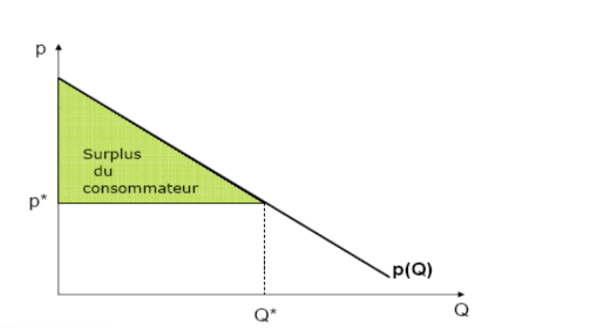
\includegraphics[scale=0.8]{Pics/surplus_consommateur.png}
\end{center}
\newpage
\section{Les défaillances du marché}
\subsection{Biens économiques}
Biens économiques : ils sont rivaux ou non, avedc un certain degré d'exclusivité
\begin{itemize}
    \item \textbf{Bien rival} : deux agents ne peuvent pas en bénéficier en même temps de ce bien \footnote{Bien rival = bien exclusif - ex : une voiture, tragédie des biens communs $\neq$ biens non-rivaux}
    \item \textbf{Bien exclusif} : bien que peut disposer l'agent que s'il paye le prix \footnote{ex : chaîne de télévision, logiciel, biens publics $\neq$ biens non-exclusifs}
\end{itemize}
Les biens et services de consommation privée traditionnelle sont les deux à la fois.
\subsection{Externalité}
C'est un effet subit par un agent économique au cours d'une action de consommation ou de production \footnote{Ces externalités sont trop ou pas assez produites, en fonciton de leurs types : il faut alors taxer et/ou subventionner certaines externalités pour les réguler.}
\begin{itemize}
    \item \textbf{Externalité positive} : effets de la R\&D, recherche publique sur la R\&d, recherche privée
    \item \textbf{Externalité négative} : effet de la pollution dûs aux rejets d'une usine
\end{itemize}
\begin{center}
    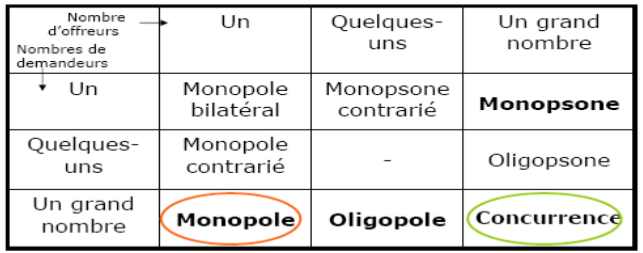
\includegraphics[scale=0.7]{Pics/defaillance_marche.png}
\end{center}
\newpage
\section{Le monopole}
\subsection{Comportement de l'entreprise}
Comportement de l'entreprise en situation de monopole
\begin{itemize}
    \item $\pi$ : profit de l'entreprise
    \item $Q(p)$ : fonction de demande
\end{itemize}
Maximisation du profit de l'entreprise, en situation de \textbf{price maker}\footnote{C'est l'entreprise qui fixe les prix}
\begin{center}
    \Large{\fbox{$max \pi(Q) = p(Q)Q - CT(Q)$}}
\end{center}
Condition de premier ordre :
\begin{center}
    \Large{\fbox{$\frac{d\pi(Q)}{dQ}=0$}}
\end{center}
\begin{center}
    \Large{$\frac{d\pi(Q)}{dQ} = \textcolor{BrickRed}{\frac{dp(Q)}{dQ}Q + p(Q)} - \textcolor{green}{\frac{dCT(Q)}{dQ}} = 0$}
\end{center}
\begin{itemize}
    \item\fbox{\textcolor{BrickRed}{$\frac{dp(Q)}{dQ}Q + p(Q) = R_{m}(Q)$}} la recette marginale \newline
    \item \textcolor{green}{$\frac{dCT(Q)}{dQ} = C_{m}(Q)$} le coût marginal \newline
    \item $\epsilon = \frac{dQ}{dp}\frac{p}{Q}$ (pour rappel)
\end{itemize}
Donc
\begin{center}
    $R_{m}(Q) = \frac{dp(Q)}{dQ}Q + p(Q) = \frac{1}{\epsilon}p(Q) + p(Q)$
\end{center}
on a alors \textbf{a l'équilibre d'une situation de monopole :}
\begin{center}
    \Large{\fbox{$R_{m}(Q) = C_{m}(Q)$}} \newline
    \textcolor{White}{.} \newline
    \Large{\fbox{$p(Q)(1+\frac{1}{\epsilon}) = C_{m}(Q)$}}
\end{center}
\newpage
Prix de monopole :
\begin{center}
    \LARGE{\fbox{$p(Q) = \frac{C_{m}(Q)}{1+\frac{1}{\epsilon}}$}}
\end{center}
En considérant la demande élastique (marché sur une échelle de temps longue soit $\epsilon \in ]-\infty;-1]$) :
\begin{center}
    \Large{$p^{M} = \frac{C_{m}(Q)}{1+\frac{1}{\epsilon}} > C_{m}(Q) = p^{C}$}
\end{center}
\begin{itemize}
    \item $p^{M}$ : prix du marché en situation de monopole
    \item $p^{C}$ : prix du marché en situation de concurrence
\end{itemize}
Marge :
\begin{center}
    \Large{\fbox{$M = \frac{p^{M}}{C_{m}}$}}
\end{center}
Taux de marge :
\begin{center}
    \Large{\fbox{$T_{m} = \frac{p^{M} - C_{m}}{C_{m}}$}}
\end{center}
\subsection{L'inefficience du monopole}
\begin{center}
    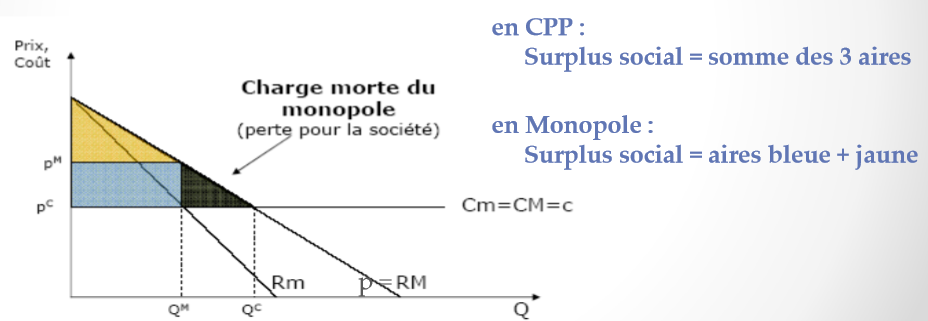
\includegraphics[scale=0.7]{Pics/Inefficience_monopole.png}
\end{center}
\newpage
\section{Les interractions stratégiques (ententes)}
Les situations de concurrence et de monopole sont deux structures de marché extrêmes et ne reflètent pas la réalité. En efft, il existe des phénomènes d'interdépendance et de startégies d'entreprises qui mènent à des ententes entres entreprises. \newline

\textbf{\textcolor{BrickRed}{Oligopole}} : nombre limité de grandes entreprises réalisant une part très importante de la production du secteur.
\newline
\begin{itemize}
    \item \textbf{Duopole de Cournot} : la quantité produite est la variable explicative de ces phénomènes \newline
    \item \textbf{Duopole de Bertrand} privilégie le prix \newline
    \item \textbf{Duopole de Stackelberg} : rôle des entreprises asymétrique (leader/follower)
\end{itemize}
\newpage
\subsection{Duopole de Cournot}
Soient deux entreprises qui produisent une quantité $q_{1}$ et $q_{2}$ de produits. Les coûts totaux sont $c_{1}q_{1}$ et $c_{2}q_{2}$. \newline
\begin{itemize}
    \item Quantité totale produite : \newline
    \textcolor{White}{.}
        \begin{center}
            \Large{\fbox{$Q = q_{1} + q_{2}$}}
        \end{center}
    \textcolor{White}{.}
    \item Fonction de demande inverse : \newline
    \textcolor{White}{.}
    \begin{center}
        \Large{\fbox{$p(Q) = p(q_{1} + q_{2}) = A - (q_{1} + q_{2})$}}
    \end{center}
    \textcolor{White}{.}
    \item Maximisation du profit de l'entreprise 1 et 2 : \newline
    \textcolor{White}{.}
        \begin{center}
            \begin{itemize}
                \Large{\fbox{$max  \pi(q_{1},q_{2}) = p(q_{1},q_{2})q_{1} - c_{1}(q_{1})$}} \newline
                \Large{\fbox{$max  \pi(q_{1},q_{2}) = p(q_{1},q_{2})q_{2} - c_{2}(q_{2})$}}
            \end{itemize}
        \end{center}
    \textcolor{White}{.}
    \item Conditions de premier ordre : \newline
    \textcolor{White}{.}
    \begin{center}
            \begin{itemize}
                \Large{\fbox{$\frac{\partial \pi_{1}(q_{1},q_{2})}{\partial q_{1}} = 0$}}
                \Large{\fbox{$\frac{\partial \pi_{2}(q_{1},q_{2})}{\partial q_{2}} = 0$}}
            \end{itemize}
    \end{center}
    \textcolor{White}{.}
\end{itemize}
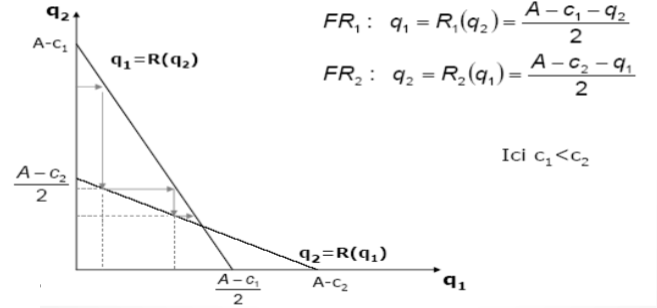
\includegraphics[scale=0.8]{Pics/Duopole_cournot.png}
\newpage
\subsection{Duopole de Bertrand}
La valeur stratégique de l'entreprise est le prix. La fonction de demande du marché $D$ s'exprime en fonction du prix $p$ fixé par les deux entreprises.
Lorsque les prix fixés sont différents, on note $\forall i \in \{1,2\}, D_{i}$ la fonction demande du marché pour l'entreprise $i$. La demande sera adressée à l'entreprise ayant le prix le plus faible.
\[
\left \{
\begin{array}{c}
    D_{1} = D(p_{1}), D(p_{2}) = 0 ;p_{1} < p_{2}\\
    D_{1} = D_{2} = \frac{D(p_{1})}{2} =  \frac{D(p_{2})}{2} ;p_{1} = p_{2}\\
    D_{2} = D(p_{2}), D(p_{1}) = 0 ;p_{2} < p_{1}
\end{array}
\right.
\]
\begin{itemize}
    \item Si $c_{1} = c_{2} = c$, la maximisation du profit $\pi_{i}$ pour les entreprises est : \newline
    \textcolor{White}{.}
    \begin{center}
        \Large{\fbox{$\pi_{i}(q_{i}) = (p_{i} - c)q_{i}$ avec $CT_{i}(q_{i}) = cq_{i}$}}
    \end{center}
    \textcolor{White}{.}
    \item Si $CT{i}(q_{i}) = c_{i}q_{i}$ et $CT{j}(q_{j}) = c_{j}q_{j}$ avec $c_{i} < c_{j}$, la maximisation du profit $\pi_{i}$ de l'entreprise i est : \newline
    \textcolor{White}{.}
    \begin{center}
        \Large{\fbox{$\pi_{i}(q_{i}) = D(c_{j})(c_{j} - c_{i})$}}
    \end{center}
    \textcolor{White}{.}
    \item Le coût moins élevé de l'entreprise 1 permet de s'accaparer la demande. La maximisation du profit pour les deux entreprises mènent à $p_{1} = p_{2} = c$. \textbf{L'équilibre de Bertrand mène au même résultats que la concurrence parfaite : profits nuls pour les entreprises à condition que les deux entreprises agissent de la même manière}
\end{itemize}
\newpage
\subsection{Duopole de Stackelberg}
Dans le cas d'un duopole de Stackelberg, une entreprise est en position dominante, \textbf{leader} et l'autre la suit, elle est \textbf{follower}. L'entreprise \textbf{leader} prend des décisions que l'autre entreprise ne peut contester et \textbf{anticipe ses réactions}. \newline
\begin{itemize}
    \item Maximisation du profit du \textbf{follower} (entreprise 2) : \newline
    \textcolor{White}{.}
    \begin{center}
        \Large{\fbox{$
        max \pi_{2}(q_{1},q_{2}) = p(q_{1},q_{2})q_{2} - c_{2}q_{2}
        $}}
    \end{center}    \textcolor{White}{.}
    \item Conditions de premier ordre : \newline
    \textcolor{White}{.}
    \begin{center}
        \Large{\fbox{$
        \frac{\partial \pi_{2}(q_{1},q_{2})}{\partial q_{2}} = 0
        $}}
    \end{center}
    \textcolor{White}{.}
    \item Fonction de réaction (identique à celle du duopole de Cournot) : \newline
    \textcolor{White}{.}
    \begin{center}
        \Large{\fbox{$
        q_{2} = R_{2}(q_{1}) = \frac{A - c_{2} - q_{1}}{2}
        $}}
    \end{center}
    \textcolor{White}{.}
    \item L'entreprise 1 connaît la façon de réagir de l'entreprise 2 : \newline
    \textcolor{White}{.}
    \begin{center}
        \Large{\fbox{$
        max \pi_{1}(q_{1},q_{2}) = p(q_{1},q_{2})q_{1} - c_{1}q_{1}
        $}}
    \end{center}
    Sachant que :
    \begin{center}
        \Large{\fbox{$
        q_{2} = R_{2}(q_{1}) = \frac{A - c_{2} - q_{1}}{2}
        $}}
    \end{center}
    \textcolor{White}{.}
    \item Conditions de premier ordre : \newline
    \textcolor{White}{.}
    \begin{center}
        \Large{\fbox{$
        \frac{\partial \pi_{1}(q_{1},q_{2})}{\partial q_{1}} = 0
        $}}
    \end{center}
\end{itemize}
\newpage
On a alors : 
\begin{center}
    \Large{\fbox{$
    q_{1} = \frac{A - 2c_{1} + c_{2}}{2}
    $}}
    \Large{\fbox{$
    q_{2} = \frac{A - 2c_{1} + c_{2}}{4}
    $}}
\end{center} 
Les quantités produites par l'entreprise 2 étant anticipées par l'entreprise 1, \textbf{l'entreprise leader peut produire plus qu'en situation de duopole de Cournot tandis que l'entreprise 2 produit moins, ce qui souligne l'avantage qu'à l'entreprise 1 sur l'entreprise 2.}
\newpage
\subsection{Entente collusive ou cartel}
Les entreprises peuvent envisager des ententes entre elles : elles forment un cartel qui se comporte comme un monopole avec plusieurs établissements et prix. \textbf{\Large{Le but est de maximiser la somme des profits des entreprises}}\newline
Ce type d'entente \textbf{n'est pas stable} : il y a généralement des non-respects de ces ententes.
\begin{center}
    \Large{\fbox{$max \pi = \pi_{1} + \pi_{2} = p(q_{1},q_{2})(q_{1} + q_{2}) - C_{1}(q_{1}) - C_{2}(q_{2})$}}
\end{center}
Conditions de premier ordre :
\begin{center}
   \fbox{\Large{$\forall i \in \{1,2\},$} \huge{$\frac{\partial \pi}{\partial q_{i}} = 0$}}
\end{center}
A l'équilibre : \Large{{$C_{m_{1}} = C_{m_{2}}$} \newline

Matrice des décisions :
\begin{center}
    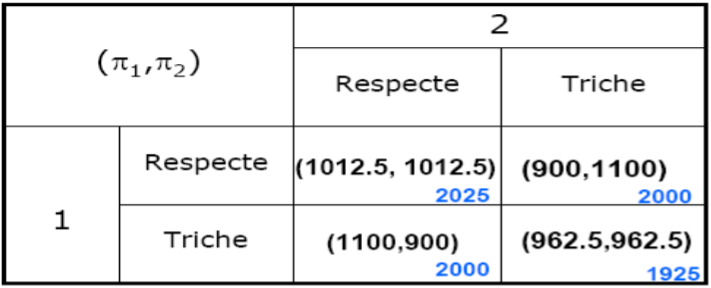
\includegraphics[scale=0.9]{Pics/Matrice_des_decisions.png}
\end{center}


\chapter*{Quelques rappels}
Rappels sur les formules de base et rappel sur le cours de traitement du signal en 1A
\begin{equation}
    \normalsize
    \tcbhighmath[fuzzy halo=0.5mm with electricultramarine!35!electricultramarine,arc=2pt,
    boxrule=0pt,frame hidden]{ 
        \lambda = cT = \frac{c}{f}
     } \nonumber
    \normalsize
\end{equation}
\begin{itemize}
    \item $c$ : célérité de la lumière ($c = 3.10^{8} m.s^{-1}$)
    \item $T$ : période en $s$
    \item $f$ : fréquence en $Hz$
\end{itemize}
Autocorrélation : \newline
\begin{itemize}
    \item \textbf{En discret} 
    \begin{equation}
        R_{xx}[k] = \frac{1}{N}\sum_{i=0}^{N}{x[i]x[i-k]}
    \end{equation}
\end{itemize}
\chapter*{Annexe 1 : démonstration de l'équation d'ondes}
\label{Annexe 1}
On considère \eqref{eq 2} \newline

Pour un fluide, la pression $P$ est fonction de la masse volumique $\rho$ tel que : $P = f(\rho)$ \newline

En se placant dans un milieu homogène constitué uniquement d'air, que l'on approxime comme un gaz parfait, on a, à l'équilibre, on a : $P_{0} = f(\rho_{0})$ \newline

La variation de pression $P_{e}$ due à la source sonore s'exprime de la manière suivante : $P_{e} =  f(\rho_{e})$ 
\footnote{Evidement $P_{e}$ est très petite devant $P_{0}$ (pour le développement de Taylor) et $P = P_{0} + P_{e} = P_{0} + k\rho_{e}$, $\rho = \rho_{0} + \rho_{e}$} \newline

On a finalement : 
\begin{align}
    P &= P_{0} +  P_{e} \nonumber \\
        &= f(\rho_{0} + \rho_{e}) \nonumber \\
    P   &\approx f(\rho_{0}) + \rho_{e}f'(\rho_{0}) \nonumber
\end{align}
On considère maintenant \eqref{eq 1} \newline

On se place au repos ($t=0$) \newline

\begin{itemize}
    \item La position $x$ sur une ligne de courant du fluide s'exprime sous la forme : $\psi (x,t)$. \newline
    \item La position voisine située en $x + dx$ s'exprime sous la forme : $\psi(x + dx,t)$. \newline
    \item La quantité de fluide par unité de surface est définie de la sorte : $\rho_{0}dx$. Avec $dx$ infinitésimal.
\end{itemize}
On obtient : 
\begin{equation}
    \psi(x + dx,t) - \psi(x,t) = \frac{\partial \psi}{\partial x}dx \Longleftrightarrow \rho_{0}dx = \rho(\frac{\partial \psi}{\partial x}dx + dx) \nonumber
\end{equation}
Comme $\rho_{e}$ négligeable devant $\rho_{0}$, on obtient : 
\begin{equation}
    \rho_{e} = - \rho_{0}\frac{\partial \psi}{\partial x} \nonumber
\end{equation}
\newpage
On considère enfin \eqref{eq 3} \newline

On prend une portion du fluide de longueur $dx$. Sa masse est $\rho_{0}dx$ et son accélération $\frac{\partial^{2} \psi}{\partial t^{2}}$. \newline

De plus, on a : 
\begin{equation}
    P_{e}(x,t) - P_{e}(x + dx,t) = \frac{\partial P}{\partial x}dx = -\frac{\partial P_{e}}{\partial x}dx \nonumber
\end{equation}
Soit : 
\begin{eqnarray}
    \rho_{0}\frac{\partial^{2} \psi}{\partial t^{2}} = - \frac{\partial P_{e}}{\partial x}\nonumber
\end{eqnarray}
\chapter*{Annexe 2 : solutions de l'équation d'ondes}
\label{annexe2}
\section{Onde Plane Progressive Monochromatique}

\section{Onde stationnaire}

\listoffigures
\listoftables

\chapter*{Bibliographie}
\begin{itemize}
    \item R. Rigal, R. Paoletti, M. Portmann, Motricit´e – approche psychophysiologique, 1974, Presses de l’universit´e du Qu´ebec (330 pages) \newline
    \item Delorme et Fl¨uckiger, Perception et r´ealit´e – Une introduction `a la psychologie des perceptions, de Boeck (517 pages) \newline
    \item E. Zwicker et R. Feldtkeller, Psychoacoustique, 1981, Masson \newline
    \item R. Feynman, Mécanique 2, 1998 (version française), Dunod \newline
    \item L. Landau et E. Lifchitz, Physique th´eorique en 10 tomes – Tome 6 – Mécanique des fluides, 1989, Librairie du globe/MIR \newline
    \item N. H. Fletcher et T. D. Rossing, The Physics of Musical Instruments, 1991, Springer-Verlag \newline
    \item A. Cuvillier, Cours de philosophie ; tome 1 ; pages 84 – 85, 541 ; 1954 ; Armand Colin \newline
    \item Emile Br´ehier, Histoire de la philosophie ; tome 3 ; pages 862 – 864 ; 1964 ; Quadrige – Presses Universitaires de France
\end{itemize}

\end{document}